\setcounter{section}{0}

\section{Complexity}
One makes computers more efficient if one 
removes the useless $0$'s between the $1$'s.\\
Here's a turing machine:
\begin{center}
  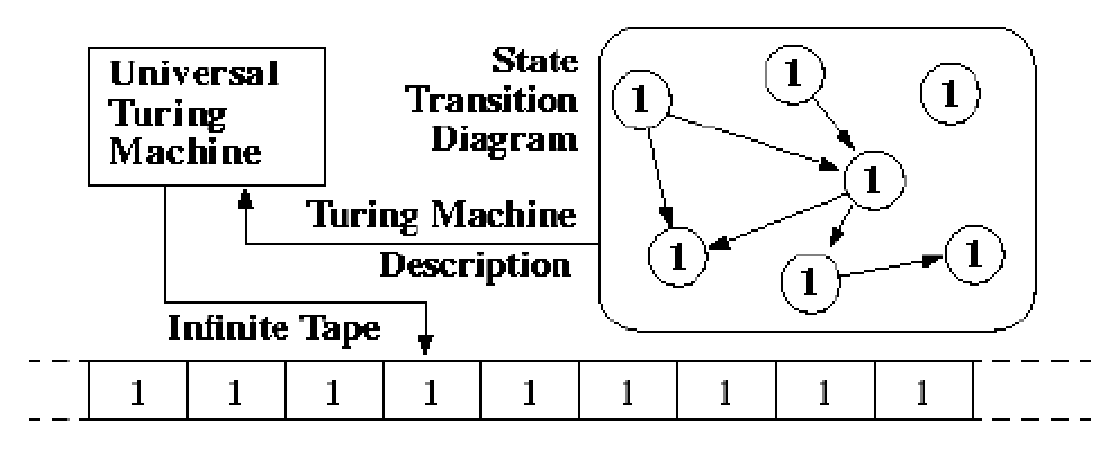
\includegraphics[width=0.9\textwidth]{turing_machine.png}
\end{center}
\begin{cor}
  The halting problem is solvable.
\end{cor}
\begin{proof}
  Halt at $1$.
\end{proof}





% draw pictures of machines whose input is something hard, and the
% output is 1.
%
% Maybe talk about halting problem?
%
%
